
\documentclass{article}
\usepackage[letterpaper,margin=1in]{geometry}
\usepackage[utf8]{inputenc}
\usepackage{enumerate}
\usepackage{bbm}
\usepackage{mathbbol}
\usepackage[algosection,ruled,lined,linesnumbered,longend]{algorithm2e}
\usepackage{algorithmic}
\usepackage{latexsym}
\usepackage{graphicx,wrapfig,xcolor}
\usepackage{float}
\usepackage{caption}
\usepackage{subcaption}
\usepackage{amssymb}
\usepackage{amsmath,amssymb,amstext,amsthm}


 \newcommand{\comment}[1]{[\begingroup\color{red!60!black}#1\endgroup]
   \marginpar{\tiny\textsc{{\color{red!60!black} To Do!}}}}

 \newcommand{\interior}{\ensuremath{\mbox{int}}} 
\newcommand{\cmd}[1]{\ensuremath{\mbox{\bf #1}}} 
\newcommand{\vio}{\ensuremath{\cmd{violation}}}
\newcommand{\st}{\ensuremath{\mbox{s.t.}}}
\newcommand{\red}[1]{\textcolor{red}{#1}}
\newcommand{\beq}{\begin{equation}}
\newcommand{\bet}{\begin{table}}
\newcommand{\eeq}{\end{equation}}
\newcommand{\real}{\mathbb{R}} %IMPORTANT
\newcommand{\htp}{\ensuremath{\mbox{HTP}}}
\newcommand{\ect}{\ensuremath{\mbox{ECT}}}
\renewcommand{\H}{\ensuremath{\mathcal{H}}}
\newcommand{\A}{\mathbb{A}}
\newcommand{\C}{\ensuremath{\mathcal{C}}}
\newcommand{\D}{\ensuremath{\mathcal{D}}}
\newcommand{\B}{\mathcal{B}}
\newcommand{\F}{\mathbb{F}}
\newcommand{\N}{\mathbb{N}} \newcommand{\R}{\mathbb{R}}
\newcommand{\T}{\mathbb{T}} \newcommand{\Z}{\mathbb{Z}}
\newcommand{\Q}{\mathbb{Q}}
\newcommand{\0}{\mathbb{0}} 
\newcommand{\1}{\mathbb{1}} 


\newtheorem{theorem}{Theorem}[section]
\newtheorem{lemma}[theorem]{Lemma}
\newtheorem{definition}[theorem]{Definition}
\newtheorem{corollary}[theorem]{Corollary}
\newtheorem{example}[theorem]{Example}
\newtheorem{nmbrs}[theorem]{Numbering}
\newtheorem{assump}[theorem]{Assumption}
\newtheorem{prop}[theorem]{Proposition}
\newtheorem{prob}[theorem]{Problem}
\newtheorem{lem}[theorem]{Lemma}
\newtheorem{thm}[theorem]{Theorem}
\newtheorem{cor}[theorem]{Corollary}
\newtheorem{rem}[theorem]{Remark}
\newtheorem{remark}[theorem]{Remark}
\newtheorem{conj}[theorem]{Conjecture}
\newtheorem{alg}[theorem]{Algorithm}
\newtheorem{ex}[theorem]{Exercise}
\newtheorem{problem}[theorem]{Problem}
\newtheorem{result}[theorem]{Result}
\newtheorem{claim}[theorem]{Claim}
\newtheorem{coroll}[theorem]{Corollary}
\newtheorem{theo}[theorem]{Theorem}
\newtheorem{defin}[theorem]{Definition}
\newtheorem{nota}[theorem]{Notation}
\newtheorem{inva}[theorem]{Invariant}

\title{Bounding the Integrality Gap of Transversal LPs}
%\author{}
%\date{May 2019}

\begin{document}

\maketitle

\section{Introduction}

Recall that a graph $H$ is a {\em minor} of $G$, if we can obtain $H$
from $G$ through a sequence of edge contractions and deletions, and
vertex deletions. In the {\em $H$-transversal} problem (\htp) one is
given a graph $G=(V,E)$, non-negative costs $c_v$, for all $v \in V$,
and a graph $H$. The goal is to find a set $S \subseteq V$ such that
$G[V\setminus S]$ has no $H$-minor.
In the following, we let $\H$
be the set of vertex subsets of $V$ whose induced subgraphs contain an
$H$-minor; i.e., $S \in \H$ iff $G[S]$ has an $H$-minor. Consider the
following natural LP relaxation of (\htp):

\begin{align}
  \min ~~ & c^Tx \tag{$\mbox{P}_{\scriptsize \htp}$}\label{lp:p} \\
  \st ~~ & x(S) \geq 1 \quad \forall S \in \H \notag \\
          & x \geq \0. \notag
\end{align}

It is not hard to see that the integrality gap of the above LP can be
large, even in special cases. For example, it is large when $H$ is a
planar graph with at least one cycle as was argued in \cite{BH+19}.
To see this, let $G$ be an $n$-vertex graph with girth $\Omega(\log n)$
and treewidth $\Omega(n)$ (e.g., certain Ramanujan graphs
\cite{Mo94}), and let $H$ be a triangle. Letting $x_v = 1/\log n$ for
all $v \in V$ is easily seen to yield a feasible solution for
\eqref{lp:p} of value $n/\log n$. On the other hand, any integral
solution for the given \htp\ instance has cost $\Omega(n)$ since
$H$-minor free graphs have treewidth $O(1)$ \cite{BH+19}. 

\section{Hitting even cycles in minor-closed graphs}

Closely related to the above is the 
{\em even-cycle transversal} problem (\ect) where
we are given a graph $G=(V,E)$, vertex costs $c_v \geq 0$ for all
$v \in V$, and where the goal is to find a min-cost set
$S \subseteq V$ such that $G[V\setminus S]$ has no even cycles. Let
\C\ be the set of even cycles in $G$. In the following, we will sometimes 
use $C \in \C$ for the set of vertices of the corresponding cycle; the meaning will be
clear from the context. 
The natural LP relaxation of \ect\ and its dual as follows:

\medskip

\hspace*{-.7cm}
\begin{minipage}{.48\textwidth}
\begin{align}
  \min ~~ & c^Tx \tag{$\mbox{P}_{\scriptsize \ect}$} \label{lp:p2} \\
  \st ~~ & x(C) \geq 1 \quad \forall C\in \C \notag \\
          & x \geq \0. \notag
\end{align}
\end{minipage}
\hspace*{1ex}
\vline
\hspace*{1ex}
\begin{minipage}{.48\textwidth}
\begin{align}
  \max ~~ & \1^Ty \tag{$\mbox{D}_{\scriptsize \ect}$} \label{lp:d2} \\
  \st ~~ & \sum_{C \in \C, v \in C} y_C \leq c_v \quad \forall v \in V
           \notag \\
          & y \geq \0. \notag
\end{align}
\end{minipage}
\medskip

Similar to the previous argument, we can show that \eqref{lp:p2} has
an integrality gap of $\Omega(\log n)$ in general. 
We suspect, however, that the LP has integrality gap $O(1)$ when $G$ is from a
minor-closed class of graphs. We will now show this for the special
case where $c=\1$. We need the following result due to Fomin, Saurabh,
and Thilikos \cite{FST11}.

\begin{theorem}\label{thm:fst}
  Let $\mathcal{G}$ be a proper minor-closed graph class and let $H$ be
  a planar graph. Then there is
  \begin{itemize}
  \item a feasible solution $U \subseteq V$ to \htp\ for $G$ and $H$, and
  \item a collection $\cal{U}$ of pairwise
    disjoint vertex subsets of $V$ each of which induces a subgraph of
    $G$ with an $H$-minor,
  \end{itemize}
  and $|U| \leq c|{\cal U}|$ for some constant $c({\cal G},H)$.
\end{theorem}

We apply Theorem \ref{thm:fst} to the given graph $G$ from some
minor-closed graph class (e.g., planar), and choose $H$ as 
the graph on two vertices with three parallel edges. The theorem
provides us with disjoint sets of vertices $D_1, \ldots, D_p$ such
that $H$ is a minor in $G[D_i]$, for all $i \in [p]$, and a set $U$ of
vertices such that $G[V\setminus U]$ has no $H$ minor. We furthermore
know that $|H| \leq cp$ for some constant $c$.

Note that $G[D_i]$ contains an $H$-minor, and hence there are vertices
$v_i$ and $u_i$ in $D_i$, and $G[D_i]$ contains three internally
vertex-disjoint $v_i, u_i$-paths. Clearly, some two of these paths
together form an even cycle $C_i$. We conclude that letting
$y_{C_i}=1$ for all $i \in [p]$ yields a feasible solution for
\eqref{lp:d2}. It is clear that $U$ may not be a feasible even cycle
transversal in $G$. 

Recall that a {\em block} in $G$ is an inclusion-wise maximal subgraph
that is either a single vertex, a bridge-edge, or a $2$-vertex
connected subgraph. We then note that $G':=G[V\setminus U]$ is
$H$-minor free, and thus a {\em cactus}; i.e., a graph in which every
block is a simple cycle, or an edge. The {\em block graph} of $G'$ is
an acyclic bipartite graph with vertex set $B_1 \cup B_2$, where $B_2$
are the blocks of $G'$, and $B_1$ are the cut-vertices. The block
graph has an edge connecting each cut vertex with any of its incident
blocks.
Let $B'_2 \subseteq B_2$ be the set of block vertices
that correspond to {\em even} cycles of $G'$. Also let $B'_1 \subseteq B_1$ be
the cut vertices with at least two neighbours in $B'_2$.  Let $\B$ be
the subgraph of the block-graph induced by the vertices in
$B'_1 \cup B'_2$. $\B$ is a forest, and we let $T_1, \ldots, T_l$ be
its trees. Let $V(T_i)=B'_{i,1} \cup B'_{i,2}$ such that $B'_{i,q}
\subseteq B'_q$ for all $i \in [l]$, and $q \in \{1,2\}$. 

W.l.o.g., we assume that $T_1,.., T_j$ are those trees in $\B$ that
have only a single node from $B'_2$ (if no such tree exists, we let $j=0$). 
For $T_i$ with $i>j$ choose a root $r \in B'_{i,1}$
and direct the edges of $T_i$ away from $r$. For each node
$a \in B'_{i,1}$, let $b(a) \in B'_{i,2}$ be an arbitrary descendant
of $a$ in $T_i$ (such a node exists by the definition of $B'_1$). 

In the following, we abuse notation mildly, and use $b(a)$, for some
$a \in B'_{i,1}$, in place of the even cycle it represents in $G'$.
We define a feasible solution $\bar{y}$ for \eqref{lp:d2} by first letting
$\bar{y}_{b(a)}=1/2$ for all $a \in B'_{j+1,1} \cup \ldots \cup B'_{l,1}$.
For $i \in \{1, \ldots, j\}$, let $C_i$ be the even cycle
corresponding to the single $B'_2$-node in $T_i$. We then let
$\bar{y}_{C_i}=1$, for all $i \in \{1, \ldots, j\}$. 
Let $\bar{y}_C=0$ for  all other even cycles. We claim that the $\bar{y}$
constructed is feasible for \eqref{lp:d2}. 
To see this, note that, by construction, no node $v \in V(G')$ is
incident to more than two even cycles with positive $\bar{y}$ value. 
In fact, if $v$ is incident to two even cycles $C_1$ and $C_2$ with
positive $\bar{y}$ value, then $\bar{y}_{C_1}=\bar{y}_{C_2}=1/2$. 

For each $1 \leq i \leq j$, let $a_i$ be an arbitrary vertex of
$C_i$. Define
\[ \bar{U} = \{a_1, \ldots, a_j\} \cup \{ a \in B'_{j+1,1} \cup \ldots
  \cup B'_{l,1} \,:\, \bar{y}_{b(a)}>0\}, \]
and note that $U \cup \bar{U}$ is a feasible solution for the
even-cycle transversal problem. Thus, letting $x_v=1$ for all $v \in U
\cup \bar{U}$, and $x_v=0$, otherwise, yields a feasible solution to
\eqref{lp:p2}. The value of this solution is no more than
$\max\{c,2\}$ times the
value of the feasible solution $y+\bar{y}$ for \eqref{lp:d2}. 
We obtain the following result.

\begin{theorem}
  Let $G$ be chosen from some minor-closed family of graphs. Then
  \eqref{lp:p2} has a constant integrality gap. 
\end{theorem}

\section{Even cycles in planar graphs}

In this section, we provide a constant-factor gap for \eqref{lp:p2} in
planar graphs in the case of general vertex costs. We will accomplish
this by refining the argument given in \cite{FJP10} for the case of
hitting {\em diamonds}.

A diamond is any sub-division of the graph consisting of three
parallel edges. In \cite{FJP10}, Fiorini et al. consider the problem
of finding a minimum-cost diamond-transversal in a general graph. The
authors show that the natural covering LP obtained from \eqref{lp:p2}
by replacing \C\ by the set \D\ of vertex sets of diamonds in $G$ has
an integrality gap of $\Omega(\log n)$. The proof is constructive and uses
a primal-dual algorithm using the natural LP and its dual.

The algorithm in \cite{FJP10} is natural and follows the well-known
primal-dual strategy: start with a pair $x=y=\0$ of infeasible primal,
and feasible dual solution. The algorithm iteratively modifies $x$,
and $y$, maintaining the fact that $x$ is $0,1$, and $y$ is dual
feasible, and stops as soon as $x$ is primal feasible. After applying
a customary {\em reverse delete} step, the algorithm arrives at a
minimally feasible solution $\bar{x} \leq x$, and the authors show
that its total cost is bounded by $O(\log n)$ times the value of dual
solution $y$. 

Somewhat more specifically, in every step of the algorithm, where $x$
is primal infeasible, we let $X$ be the vertex set corresponding to
$x$. The algorithm then carefully chooses a diamond $D$ in
$G[V\setminus X]$, and increases its dual variable $y_D$ as much as
possible, maintaining dual feasibility. At this point, the dual packing
constraint for a vertex $v \in V\setminus X$ becomes tight, and the
algorithm sets $x_v=1$. Once $x$ is feasible for the LP, the algorithm
computes a {\em minimal} feasible solution $\bar{x} \leq x$, and the
authors show that $y_D > 0$ only if $|D \cap \bar{X}| =  O(\log
n)$. This suffices to prove that $\bar{X}$ is an $O(\log
n)$-approximate diamond hitting set. 

In this
section, we show that their algorithm can be simplified in the case of
even cycles, and that it can be strengthened using the planarity of
the underlying graph.

\subsection{Ideas and a first attempt}

A key first observation is captured in the following Lemma which is a
special case of Kotzig's Theorem on Light Planar Subgraphs (e.g., see
Section 3 of \cite{JV13}). 

\begin{lemma}\label{discharge}
  A planar multigraph $ G=(V,E)$ where every vertex has at least 3
  distinct neighbours and no faces of length 2 contains 2 adjacent
  vertices whose degrees sum to at most 13.
\end{lemma}

In particular, the above lemma has the following consequence:

\begin{cor}\label{cor:smallec}
  A 2 connected planar graph G of minimum degree 3 and no faces of
  length 2 contains an even cycle with at most 11 edges.
\end{cor}

\begin{wrapfigure}{r}{0.3\textwidth}
  \begin{center}
    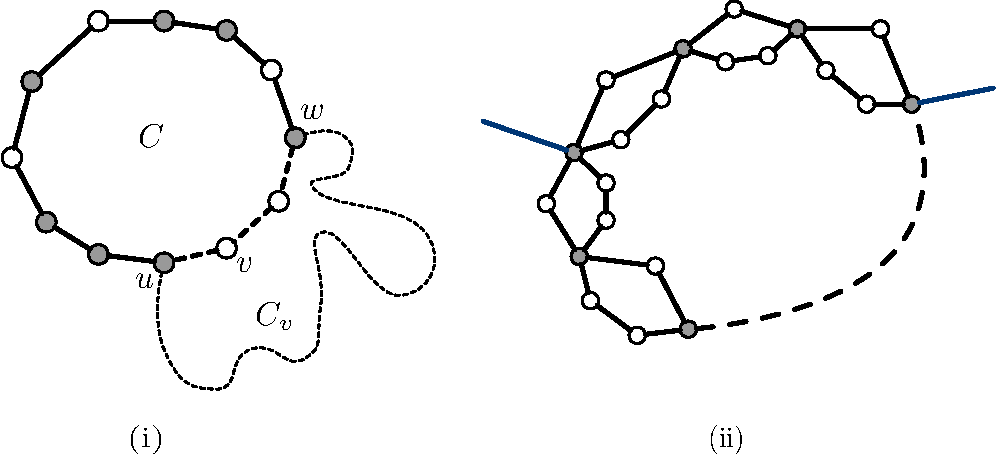
\includegraphics[width=.3\textwidth]{simple-pd.pdf}
  \end{center}
  \caption{\label{fig:simplepd} The figure shows even cycle
    $C$. White vertices are contracted during compression and have
    degree 2 in $G[V\setminus X]$, grey vertices have degree at least
    3 in the same graph.}
\end{wrapfigure}

Hao's notes have a self-contained proof of the above two statements.
From here, our algorithm follows the ideas provided in \cite{FJP10},
simplifying and adapting to even cycles where possible. 

Corollary \ref{cor:smallec} suggests the following natural algorithm:
start with $X=\emptyset$, and $y=\0$. At any point in the algorithm
where $X$ is not feasible, compute the {\em 1-compression} $G_1$ of
$G[V\setminus X]$ as follows: as long as $G$ has a node $v$ of degree 2 with
exactly two neighbours $u$ and $w$ in $G$, {\em contract} $v$; i.e.,
replace $uv$ and $vw$ by $uw$, and delete $v$. In the resulting graph
$G_1$, all nodes have degree at least $3$. Now find a cycle $C_1$ in
$G_1$ of length at most $11$ whose corresponding cycle $C$ in $G$
(which we will also call the {\em projection} of $C_1$ in $G$)
is
even. Increase $y_C$ as much as possible, and add the newly tight
vertices to $X$. Repeat the above until $X$ is feasible, then run
reverse delete, and obtain a minimally feasible set $\bar{X}$. Note
that the minimality of $\bar{X}$ implies that, for all
$v \in \bar{X}$, there is an even {\em witness} cycle $C_v$ in $G$
that that $C_v \cap \bar{X} = \{v\}$. More precisely,  there is such a
witness cycle $C_v$ that is in the projection of  the compressed
residual graph {\em at the time} when $v$ was chosen. 

\begin{lemma} \label{lem:simplealg}
  Suppose that the above algorithm terminates with
  feasible solution $\bar{X}$. Then the total cost of $\bar{X}$ is at
  most $11$ times the value of the computed dual solution.
\end{lemma}
\begin{proof}
  Let us consider an even cycle $C$ with $y_C>0$, and let $C_1$ be the
  short cycle in the 1-compression $G_1$ of the graph $G[V\setminus
  X]$ at the time where $y_C$ was increased. 
  In Figure
  \ref{fig:simplepd}, white nodes have degree $2$ in $G[V\setminus
  X]$, and grey nodes have degree at least three. Hence the cycle
  depicted has length $7$ in $G_1$. Suppose that $v \in V(C) \cap
  \bar{X}$ is a node on $C$ that was chosen by our algorithm for the
  final transversal.

  Consider two adjacent nodes $u$ and $w$ in $V(C_1)$, and let
  $P_{uw}$ be the corresponding path in $G$. 
  Let us first assume that $v$ is an internal (degree $2$) node of
  $P_{uw}$ for two adjacent nodes $u,w$ of $V(C_1)$. In this case,
  note that the witness cycle $C_v$ of $v$ contains all nodes of
  $P_{uw}$ including $u$ and $w$ themselves. Thus, if $\bar{X}$
  contains $v$ then it contains no other nodes from $P_{uw}$.

  Now suppose that $v \in \bar{X} \cap C_1$ is node of
  degree at least three on $C$, and let $u$ and $w$ be the neighbours
  of $v$ on $C_1$. Using the same argument as before, we see that
  no internal vertex of $P_{uv}$ and $P_{wv}$ can be in $\bar{X}$ in
  this case. Hence, we must have
  $|\bar{X} \cap C| \leq 11$, and the solution
  $\bar{X}$ has cost no more than $11\sum_Cy_C$. 
\end{proof}

\begin{wrapfigure}{r}{0.3\textwidth}
  \begin{center}
    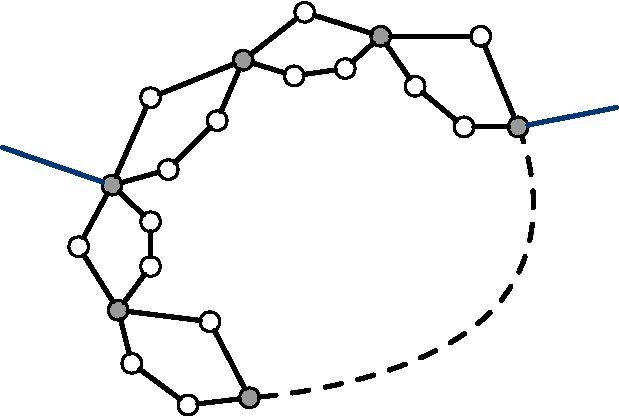
\includegraphics[width=.3\textwidth]{longcyc.pdf}
  \end{center}
  \caption{\label{fig:longcyc} A graph in which every even cycle is long.}
\end{wrapfigure}

Unfortunately, the above algorithm does not always terminate. The
reason is that we may not be able to find an even cycle whose
1-compression has at most 11 edges. Consider for example the 
graph depicted in Figure \ref{fig:longcyc}. This graph has many even
cycles, albeit no short ones! Notice that the compression of this
graph has faces of length $2$, and hence Corollary \ref{cor:smallec}
does not apply. 

\subsection{Dealing with graphs without even cycles of small
  compressed length}

Consider vertex sets $C'_1$ and $C'_2$ that each contain the  vertex set of an even cycle
in $G$; i.e., for $j \in \{1,2\}$, there is an even cycle $C_j \in \C$ such that $C_j
\subseteq C'_j$. 
Define $a_v^{C'_1,C'_2}=1$
for all $v \in (C'_1 \cap C'_2)$, $a_v^{C',C'}=1/2$ for
$v$ in the symmetric difference $C'_1\setminus C'_2 \cup C'_2 \setminus C'_1$
of $C'_1$ and $C'_2$, and
$a_v^{C'_1,C'_2}=0$, otherwise. Note that the following inequality is
dominated by the two original cover inequalities for
sets $C_1$ and $C_2$:
\[ \sum_{v} a^{C'_1,C'_2}_v x_v \geq 1. \]
Hence, we obtain a new
pair of LPs that are equivalent to \eqref{lp:p2} and its
dual. Here, we abuse notation, and let \C\ now be the set of pairs $(C'_1,C'_2)$ where
$C'_1$ and $C'_2$ are (not necessarily disjoint nor different) 
supersets of even cycles in $G$.

\medskip

\hspace*{-.7cm}
\begin{minipage}{.48\textwidth}
\begin{align}
  \min ~~ & c^Tx \tag{$\mbox{P}_{\scriptsize \ect}$} \label{lp:p3} \\
  \st ~~ & \sum_{v \in V}a^{C'_1,C'_2}_vx_v \geq 1 \quad \forall 
  (C'_1,C'_2) \in \C \notag \\
          & x \geq \0. \notag
\end{align}
\end{minipage}
\hspace*{1ex}
\vline
\hspace*{1ex}
\begin{minipage}{.48\textwidth}
\begin{align}
  \max ~~ & \1^Ty \tag{$\mbox{D}_{\scriptsize \ect}$} \label{lp:d3} \\
  \st ~~ & \sum_{(C'_1,C'_2) \in \C} a^{C'_1,C'_2}_vy_{C'_1,C'_2} \leq c_v \quad \forall v
  \in V
           \notag \\
          & y \geq \0. \notag
\end{align}
\end{minipage}
\medskip

Note that the original cover inequalities for even cycles 
$C$ are contained in the reformulation of \eqref{lp:p2}, by
letting $C'_1=C'_2=C$. For convenience we will write
$y_C$ in place of $y_{C,C}$ from here on. 

Our algorithm maintains a pair $(x,y)$ of (partial) primal,
and dual solutions for the above pair of LPs; for convenience, we let $X$ be the set of vertices
corresponding to incidence vector $x$. 
At any time, the algorithm will consider the 1-compression $G_1$
of the graph $G[V\setminus X]$. The algorithm works as before if $G_1$
contains a simple, short cycle (i.e., a cycle without parallel edges, and length no more
than 11) whose
projection in $G$ is an even-length cycle $C$. In this case we
increase the dual variable $y_{C}$ as described in the previous
section as much as possible, adding newly tight vertices to set $X$. 

Note that the same argument also works if there is a pair of vertices $u$ and $v$ that are connected
by at least three edges $e_1$, $e_2$, and $e_3$ in $G_1$. In this case, two of these edges, say
$e_1$ and $e_2$, project to an even length cycle $C$ in $G$. We proceed as before.

From here on, we assume that $G_1$ has at most two edges connecting every pair of vertices. 
We also assume, w.l.o.g., that every edge of $G_1$ is contained in some cycle with even projection,
and therefore, $G_1$ is 2-connected. Assume now that $G_1$ has cycles with even projection, but none
that are short and simple. In this case, Corollary \ref{cor:smallec} implies that $G_1$
cannot be simple. 

\begin{figure}[ht]
  \begin{center}
    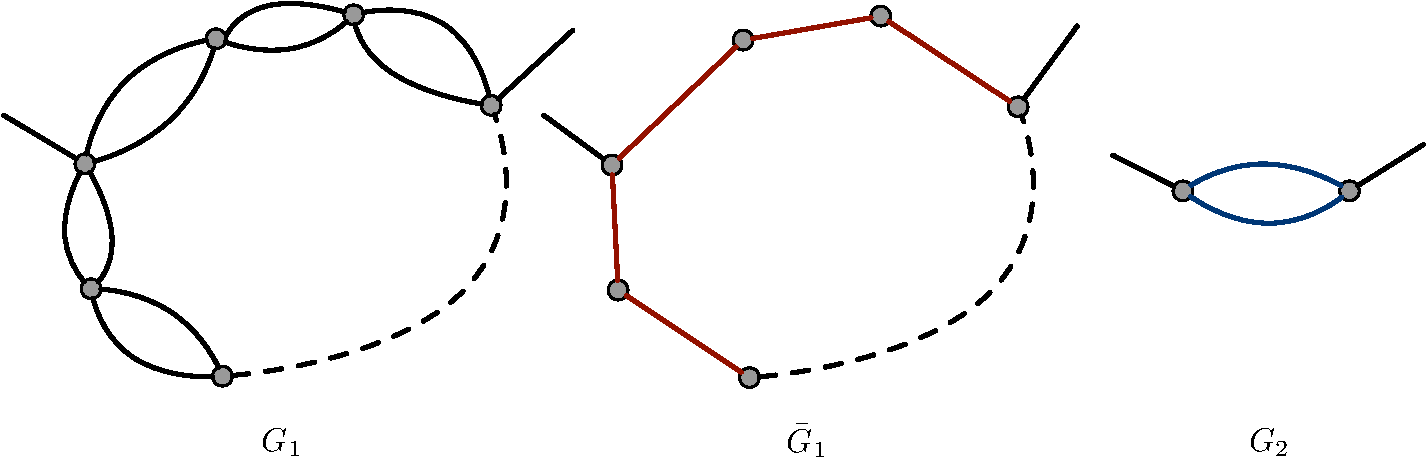
\includegraphics[width=.85\textwidth]{2compress.pdf}
  \end{center}
  \caption{\label{fig:2compress} The figure shows 1 and 2-compression
    $G_1$ and $G_2$ of the graph shown in Figure \ref{fig:longcyc}. In $\bar{G}_1$ we replace parallel
    edges in $G_1$ by twin edges. }
\end{figure}

We obtain graph $\bar{G}_1$ from $G_1$ by replacing each pair of parallel edges
connecting vertices $u$ and $v$ by a single {\em twin} edge $uv$.
Note that each face in this new graph has length at least 3.
Obtain the 2-compression $G_2$ of
$G$ by contracting degree-2 nodes in $\bar{G}_1$; see Figure
\ref{fig:2compress}. In the following, abusing notation slightly, we
call edges created by contracting vertices in $\bar{G}_1$ {\em
twin} (as their projection in $G_1$ must contain twin edges). Using $G_2$, we will now
identify a certain even {\em cycle} whose dual variable we increase. 
We branch into two
cases. 

\paragraph{$G_2$ is simple.}

We first assume that any pair of vertices is connected by at most 1 edge in $G_2$. 
In this case, Corollary \ref{cor:smallec} implies that $G_2$ has an even cycle $C_2$ 
of length at most $11$. Since $G_1$ does not have a short, simple cycle with even
projection, it follows that $C_2$ must contain at least one twin edge.

We now focus on an edge $uv$ on $C_2$, and let $\bar{P}_1$, $P_1$, and $P$
be its projections in graphs $\bar{G}_1$, $G_1$, and $G$, respectively.  
Following the notational conventions of 
\cite{FJP10}, we say that $P$ is the {\em piece} corresponding to $uv$. 
Note that the piece of a non-twin edge $uv$ is a $u,v$-path whose
internal nodes have degree $2$ in $G[V\setminus X]$.

If $uv$ is a twin edge of $C_2$, then the path $\bar{P}_1$ consists of twin, and non-twin
edges. In turn, a twin edge $u'v'$ on $\bar{P}_1$ projects to a
subgraph of $G[V \setminus X]$ that is induced by two internally vertex
disjoint $u',v'$-paths $S_1$ and $S_2$. Furthermore, concatenating these two
$u',v'$-paths yields an odd cycle. 

In summary, one now sees that
the {\em block-graph} of the projection of twin edge $uv$ of $C_2$ is 
a path in $G[V\setminus X]$. Moreover, the
blocks in this subgraph are odd cycles; see Figure \ref{fig:cycG2} for
an example.

\begin{figure}[b]
  \begin{center}
    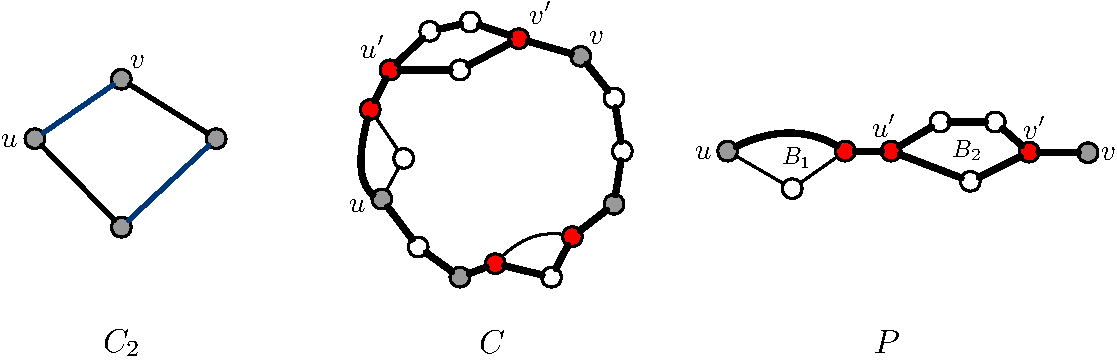
\includegraphics[width=.8\textwidth]{cycG2.pdf}
  \end{center}
  \caption{\label{fig:cycG2}The first two figures show a  short cycle $C_2$ in $G_2$, and its
    corresponding projection in $G$. The right figure above shows the piece
    of twin edge $uv$ of $C_2$. Note the thick edges of cycle $B_2$ above: these
    are type-3 edges.}
\end{figure}

Let us focus on a piece $P$ corresponding to a twin edge $uv$ of
$C_2$. Vertices $w \in V(P)\setminus  \{u,v\}$ have degree $2$ in
$G_1$, or they are {\em cut-vertices} of $P$, and have degree $2$ in
$\bar{G}_1$. In Figure \ref{fig:cycG2} we have coloured such vertices
in red.
In the following, we keep track of the 
{\em slack} in the dual constraint of each vertex $v$ for the current dual feasible
solution for \eqref{lp:d3}:
\[ \bar{c}_v := c_v - \sum_{(C'_1,C'_2) \in \C} a^{C'_1,C'_2}_vy_{C'_1,C'_2}.\]
We now define a {\em canonical} subgraph of each piece $P$. 
This subgraph will be the support of the inequality of \eqref{lp:p3} whose dual variable
we want to increase. The subgraph is induced by a set of vertices 
that we classify as {\em type-1}  
{\em type-2}, or {\em type-3}.

For a non-twin edge
$uv$ of $C_2$ we let all vertices of the corresponding piece $P$ be of type 1. 
Now consider a twin-edge $uv$ of $C_2$. All vertices of $P_1$ are added as type-1. 
Let $u'$ and $v'$ be two neighbouring vertices on $P_1$ that are connected by twin edges 
$e_1$ and $e_2$ in $G_1$ (see Figure \ref{fig:cycG2}). 
Let $S_1$ and
$S_2$ be the paths in $G[V\setminus X]$ corresponding to $e_1$ and
$e_2$, respectively. We let the residual cost $\bar{c}(S)$ of a path $S$ be the
smallest residual cost of any of its internal nodes. 
If the maximum among $\bar{c}(S_1)$ and $\bar{c}(S_2)$ is unique, then let the vertices
of the maximizer be of type 1. Otherwise label $u'$ and $v'$ type-1, and make all internal
vertices of $S_1$ and $S_2$ type-2. We will call the vertices of $S_1$ and $S_2$ together
with $u'$ and $v'$ a {\em type-2 cycle} in this case.

Suppose first that the number of type-2 cycles over all pieces of $C_2$ is
odd. In this case, pick an arbitrary such cycle and label all its internal
vertices type-3. We call the corresponding cycle a {\em type-3 cycle}. For any
$v \in V$, we now let
\[
  a_v = \begin{cases} 
    1 & \mbox{if $v$ is type-1, or type-3}\\
    1/2 & \mbox{if $v$ is type-2}\\
    0 & \mbox{otherwise.}  
    \end{cases}
\]
We claim that the inequality
\begin{equation}\tag{$\circledast$}\label{eq:star} 
  \sum_v a_v x_v \geq 1 
\end{equation}
is part of \eqref{lp:p3}. To see this, let us assume that the number of type-1
vertices is even (the subsequent argument is easily adapted if this number is
odd). Let $\bar{C}^1, \ldots, \bar{C}^{2q}$ be the even cardinality set of all
type-2 cycles over all pieces of $C_2$. Furthermore, for $1 \leq i \leq 2q$,
let $ \bar{S}^i_1$ and $\bar{S}^i_2$ be the internal vertices of the two paths
defining $\bar{C}^i$. Since $\bar{C}^i$ is odd by assumption it follows that
$\bar{S}^i_1$ and $\bar{S}^i_2$ have different parity. By possibly
renumbering, we may therefore assume that the parity of $\bar{S}^{2i}_1$ is
different from that of $\bar{S}^{2i+1}_1$, for all $1 \leq i \leq q$. 

Assume first that there are no type-3 vertices. In this case, we obtain two
even cycles, by adding the set of type-1 vertices to  
\[ Q_j =
\bigcup_{i=1}^q(\bar{S}^{2i}_j \cup \bar{S}^{2i+1}_j), \]  
for $j=1,2$. 
Assume, on the other hand, that there are type-3 vertices, and let $S_1 \cup S_2$ be the
corresponding partition of the internal vertices of the paths defined above. 
We now see that adding the set of type-3 vertices to $Q_j$ yields the superset
of an even cycle, for $j=1,2$. This now completes the argument that \eqref{eq:star} is
part of \ref{lp:p3}. 

The algorithm increases the dual variable $y_{\circledast}$ corresponding to
inequality \eqref{eq:star} as much as possible, while maintaining dual feasibility. 
We then add tight vertices to $X$. Note that our definition of $a$ and inequality 
\eqref{eq:star} allows us to maintain the following invariant.

\begin{inva}\label{inva}
  Consider a twin edge $e_1$ and $e_2$ in $C_1$ as defined above, and let $S_1$ and $S_2$
  be the corresponding vertex sets in $G[V\setminus X]$. If $\bar{c}(S_1) \geq \bar{c}
  (S_2)$ before the increase of $y_{\circledast}$ then this will be true also after the
  increase, and until the end of the algorithm's execution. 
\end{inva}

Let $S_1 \cup S_2$ be the set of internal vertices of a type-2 or type-3 cycle. Note that
Invariant \ref{inva} implies that if the dual constraint of some $v_1 \in S_1$ becomes
tight in a step of the algorithm, then there is a vertex $v_2 \in S_2$ whose dual
constraint becomes tight at the same time. For such a tight cycle, we pick exactly two
vertices
$v_1$ and $v_2$ in $S_1$ and $S_2$, respectively, and add them to $X$. We will later refer
to such an addition as a {\em type-2/3 addition}.

\paragraph{$G_2$ is not simple.}

In this case, $G_2$ has two vertices $u$ and $v$ that are connected by at least two edges
$e_1$ and $e_2$. By assumption $\bar{G}_1$ is a simple graph. Thus, at least one of $e_1$
and $e_2$, say $e_1$, is a twin edge. In this case we let $C_2$ be the cycle formed by
$e_1$ and $e_2$ and proceed as above.

\paragraph{When the algorithm terminates.}

The algorithm terminates at the first time when $X$ is a feasible solution to \ect. We
then obtain a minimal feasible solution $\bar{X}$ through a reverse-delete step. 
Suppose that reverse delete considers vertices $v_1$ and $v_2$ that were part of a
type-2/3 addition in the algorithm. Note that if reverse delete decides to remove one of
these vertices, then it will remove both. 

\section{Analysis}

Let $y$ be the final feasible dual solution computed by the algorithm. 
Our goal is to prove that the computed solution is $12$-approximate. 
Following the classic primal-dual argument, it
suffices to show that
\begin{equation}\label{eq:pd}
\sum_{v \in \bar{X}} a^{C'_1,C'_2}_v \leq 12,
\end{equation}
whenever $y_{C'_1,C'_2}>0$. The inequality follows from the argument used in Lemma 
\ref{lem:simplealg} in the case where $C'_1=C'_2=C$ for some even cycle $C \in \C$
(e.g., this is the
case when our algorithm found a simple, short, even cycle in $G_1$).

So let us consider the situation during the algorithm where no such short, simple, even
cycle exists, but where $G[V\setminus X]$ still has even cycles. 
In this case, as described above, our algorithm computes the 2-compression $G_2$ of $G
[V\setminus X]$ and finds a short cycle $C_2$ whose projection $C$ in $G[V\setminus
X]$ contains an even cycle. In the construction of inequality \eqref{eq:star}, the
algorithm selects
type-1, type-2, and type-3 vertices in $C$.
We will show that the sum of the $a$-coefficients of
the internal vertices of $P \cap \bar{X}$ and any one of $u$ and $v$ is at most $1$ if $P$
has no type-3 vertices, and at most 2 otherwise. Inequality 
\eqref{eq:pd} then follows from the fact that at most one piece of $C_2$ has type-3
vertices by construction. 

Consider first the case where $uv$ is a non-twin edge of $C_2$, and recall that its
piece $P$ is a path whose internal vertices have degree $2$. As in the proof of Lemma 
\ref{lem:simplealg}, at most one of the internal vertices of $P$ can be in $\bar{X}$.
Similarly, if
one of $P$'s endpoints is in $\bar{X}$ then none of the internal vertices can be in
$\bar{X}$.

\begin{figure}
  \begin{center}
    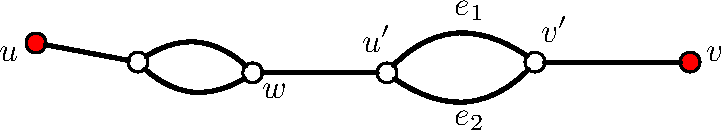
\includegraphics[width=.5\textwidth]{piece.pdf}
  \end{center}  
  \caption{\label{fig:piece} The figure shows the projection $P_1$ of a piece of an
  edge $uv$ on an even
  cycle $C_2$ in $G_2$.}
\end{figure}  

In the remaining part of the proof, we consider a twin edge $uv$ on $C_2$ with
projections $P_1$ in $G_1$, and $P$ in $G[V\setminus X]$; we refer the reader
to Figure \ref{fig:piece} for an example.

\paragraph{Case 1: $P$ has no type-3 vertices.}

As in the proof of Lemma
\ref{lem:simplealg}, $\bar{X}$ has at most one of the internal nodes of $P_1$, and if
there is such a node, then $P$ contains no other node of $\bar{X}$. In this case, 
the sum of $a^{C'_1,C'_2}_v$ over the nodes of $P \cap \bar{X}$ is at most 1.
So suppose that $\bar{X}$ has none of the internal vertices of $P_1$. 

Focus, on a pair of twin edges $e_1$ and $e_2$, connecting vertices $u'$ and
$v'$ of $P_1$, and as before, let $S_1$ and $S_2$ be the vertex sets of the
projections of these edges.  Suppose that the residual cost of $S_1$ is at
least that of $S_2$. Then by Invariant \ref{inva}, and by the way we perform
reverse-delete, $\bar{X}$ contains a vertex from $S_1$
only if it also contains a vertex of $S_2$. If $S_1 \cup S_2$ forms a type-2/3 cycle, then
a stronger condition holds: $\bar{X}$ contains either exactly two vertices $v_1 \in S_1$,
and $v_2 \in S_2$, or $(S_1 \cup S_2)\cap \bar{X}=\emptyset$. 
%Moreover, the piece $P$
%contains at most one type-2/3 cycle with  non-empty intersection with $\bar{X}$. 

Let us first assume that $\bar{X}$ contains
vertices from both $S_1$ and $S_2$. In this case, by the familiar witness cycle
argument, we see that these two vertices are the only vertices in $P \cap
\bar{X}$. If $S_2$ is in the support of \eqref{eq:star} then it must be that
the projection of $e_1$ and $e_2$ forms a type-2 cycle. Thus, the sum of the
$a$-coefficients of the two $\bar{X}$-vertices in $S_1 \cup S_2$ is $1$ in
this case. On the other hand if $e_1$ and $e_2$ do not form a type-2 cycle,
then $S_2$ is not in the support of \eqref{eq:star}, and hence the sum of
$a$-coefficients of vertices in $P$ is at most $1$ in that case as well. 

Let us now assume that for all cycles $S_1 \cup S_2$ of piece $P$, $\bar{X}$
contains at most one vertex from $S_1 \cup S_2$. Thus, if $\bar{X} \cap S_2
\neq \emptyset$ we must have $\bar{X}\cap S_1=\emptyset$ for such a cycle. But
this implies that we must have had $\bar{c} (S_1)>\bar{c}(S_2)$ at the time of
increase, and hence $a(S_2)=0$. 

\paragraph{Case 2: $P$ has type-3 vertices.}

Let $S_1,S_2$ be the vertex set of the type-3 cycle. By the same argument as before, 
$\bar{X}$ contains none or two vertices from $S_1 \cup S_2$. If it contains none, then the
argument of the previous case applies and the sum of $a$ coefficients of $P$ vertices is
at most $1$. Otherwise, $P$ contains exactly these two vertices from $\bar{X}$, and the
$a$ coefficients of $P$ vertices sum to $2$. Since at most one piece of $C_2$ can contain
type-3 vertices, we now obtain the following theorem. 

\begin{theorem}
  The above algorithm is $12$-approximate. 
\end{theorem}

We can get an 11 approximation by using a stronger version of Corollary \ref{cor:smallec}
that is specifically tunes for our application. In the following, let $G_2$ be the
2-compression of a given planar graph $G$. As before, we assume that $G_2$ is 2-connected.

\begin{corollary}
Suppose that $G_2$ has no faces of length 2. Then (a) it contains an even cycle without
twin edges of length at most $11$, or (b) it contains a cycle $C$ that contains a twin
edge of
length no more than $10$. 
\end{corollary}
\begin{proof} 
If $G_2$ has a parallel edge, one of which is twin, then we get an even cycle with at most 3 pieces.
By lemma \ref{discharge} we can find adjacent faces $f_1,f_2$ of $G_2$ whose lengths sum
to at most 13. If one of the faces has a twin edge, then the corresponding cycle satisfies
condition (b) above. Otherwise, the union of $f_1$ and $f_2$ contains an even cycle
without twin edges of length at most $11$, and hence (a) holds. 
\end{proof}

One can improve the 11-approximation by noting that getting 11 pieces in our
even cycle only happens in a very specific case. In the proof of Lemma
\ref{discharge} which guarantees an edge $uv$ where the degrees of $u,v$ sum
to at most 13 it must be that no edges incident to the chosen vertex were
added when we looked for an edge maximal counterexample. Further it must be
that at most 1 neighbour of $v$ ($\deg(v)>\deg(u)$) which has degree less than 6
has degree 4.  For the next part let us keep one hit node in the interior of
each piece and delete the rest we will prove in the remaining graph that our
even cycle contains at most 9 hit nodes. Given an edge $uv$ in $G$ let
$p(u,v)$ denote the piece in $G$. 

\begin{remark}\label{consecutive}
Let $ tv_iv_{i+1} $ be a triangle face of $G_2$ which has odd in $G$ with no twin edges. Let $ v_{i-1} $ be a neighbour of $v_i$, and $v_{i+2}$ a neighbor of $v_i$. Suppose that $v_i,v_{i+1}$ have no other neighbors. Then  $ p(v_{i-1} , v_i ) \cup p(v_i,v_{i+1} ) \cup p(v_{i+1},v_{i+2} ) $  contains fewer than 3 hit nodes.
  % Let  non twin edge distinct from $ v_1 v_3 $ , let $ v_i t_i v_{i+1}$  be the triangle face  using $v_i, v_{i+1} $ if each of $v_i, v_{i+1}$ is incident to exactly 3 faces. 
\end{remark}
%%\begin{proof}
% Suppose that $ p(v_{i-1} , v_i ) \cup p(v_i,v_{i+1} ) \cup p(v_{i+1},v_{i+2} ) $ contains 3 hit nodes, let $w$ be the  "middle" hit node, then each of $ p(v_{i-1} , v_i ) ,p(v_{i+1},v_{i+2} ) $ contains a hit node besides w. Let $A_w$ be a witness cycle for $w$ and consider the subpath $ Q_w$ of $A_w$ containing $w $ and lying in $ p(v_{i-1} , v_i ) \cup p(v_i,v_{i+1} ) \cup p(v_{i+1},v_{i+2} ) $  such a path cannot use the pieces $ p(v_{i-1} , v_i ) ,p(v_{i+1},v_{i+2} ) $  and hence both ends of the path are  $t_i$ and so this cycle is $A_w$, but by assumption this cycle is odd in $H$ a contradiction.  \\
 %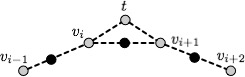
\includegraphics[scale=0.3]{ConHitnode.jpg}
%\end{proof}














\bibliography{main}
\bibliographystyle{plain}
\end{document}
